\chapter{Physical Simulations}\label{chapter:physical-simulations}
Modeling the world around us is a longstanding problem of science. For many
physical processes, model equations exist, describing how a given system evolves
through time. From weather and climate forecasts (\cite{stocker2014climate})
over quantum physics (\cite{QuantumSim}), to the control of plasma fusion
(\cite{PlasmaControl}), or optimizing the shape of
vehicles (\cite{OptimizationCFD}), it has become an integral part of engineering
applications to use numerical methods to derive solutions from model equations.

In this section, we build up an understanding of modeling physical phenomena
with \acfp{PDE}. We also introduce the notion of \acf{DP} after a brief
introduction to classical numerical methods.

\section{Partial Differential Equations}
\acp{PDE} are the most fundamental description of evolving systems from quantum
mechanics to turbulent flows. \acp{PDE} are equations relating the partial
derivatives of some unknown function. For a physical system $\vb{u}(\vb{x},t)$,
the governing \ac{PDE} can be written as

\begin{equation}
\label{eq:pde}
\pdv{\vb{u}}{t} = \mathcal{P}\left(\vb{u}, \pdv{\vb{u}}{\vb{x}},
\pdv[2]{\vb{u}}{\vb{x}},\dots,\vb{y}(t)\right),
\end{equation}
where $\mathcal{P}$ models the physical behavior of the system, and $\vb{y}(t)$
denotes an (optional) external force factor. 

\subsection{Numerical Methods}
Analytic solutions (i.e. closed-form expressions) can be found only for a very
small subset of \acfp{PDE}. The main idea behind numerical methods is to
discretize an equation, reducing a continuous equation (such as \ref{eq:pde}) to
a finite number of unknowns. We discretize the temporal dimension by introducing
a step time $\Delta t$. For spatial dimensions, a typical solution is discretizing
on by assigning values to grid cells or particles: we call these Eulerian, and
Lagrangian perspective, respectively.

\subsubsection*{Numerical Integration with Explicit Schemes}
As we introduce only a small subset of numerical methods, we refer to
\cite{Baraff1997PhysicallyBM} to give an introduction to numerically
approximating \acfp{PDE} from a computer graphics perspective for use in
physically based modeling. They discuss the respective shortcomings of the
techniques in a visual way.

Euler's method (introduced back in 1768) starts with an initial value, and steps
along the tangent of the function. Given a first order \acf{ODE} 
$$\dv{x(t)}{t} = f(x,y)$$ describing the derivative of a function $x(t) = y$,
and starting with an initial condition $x_0$, $y_0$, and step size
$\Delta t$ at time $t_0$,
an Euler step 
$$y_1 = y_0 + \Delta t f(x_0, y_0)$$
gives the $y_1$ estimation for $x(t_0 + \Delta t)$. With this, we can compute
$f(x_1, y_1)$ and so on, giving us an estimated trajectory for $x(t)$. Note that
$y_n \neq x(t_0 + n \Delta t)$, as the function $x(t)$ is unknown. 

Euler's method gives us a first order approximation of the function. The
\textit{midpoint method} achieves second order accuracy by evaluating the
derivative at an intermediate half step:
\begin{align*}\label{eq:midpoint}
  \tilde{y} &= y_0 + \frac{\Delta t}{2} f(x_0, y_0) \\
  y_1 &= y_0 + \Delta t f(x_0+ \Delta t /2, \tilde{y}).
\end{align*}

The midpoint is actually a $2^{nd}$ order \acf{RK} method. The \ac{RK}
family of integrators can be used to construct integrators of arbitrary order.
In practice, the $4^{th}$ order \ac{RK} gives a good compromise between accuracy
and computation cost:
\begin{align*}
  k_1 &= f(x_0, y_0) 
      &\qq*{(compute a first estimate of the slope)}\\
  k_2 &= f(x_0+\Delta t/2, y_0+\Delta t / 2 k_1) 
      &\qq*{(predict the tangent at midpoint)}\\
  k_3 &= f(x_0+\Delta t/2, y_0+\Delta t / 2 k_2) 
      &\qq*{(correct the estimate)}\\
  k_4 &= f(x_0+\Delta t, y_0+\Delta t k_3) 
      &\qq*{(predict slope with full step)}\\
  y_0 &= y_0 + \frac{1}{6}(k_1 + 2k_2 + 2k_3 + k_4) 
      &\qq*{(finally, perform step with weighted slopes).}
\end{align*}

Choosing a good $\Delta t$ is very important for these explicit integration
techniques to prevent instability problems, and give reasonable accuracy. 

\subsubsection*{Spatial Discretization}
\todo{
  Finite Differences:
  \begin{itemize}
    \item Replace domain by a finite number of discrete points.
    \item These points are typically located on Eulerian grid.
    \item Discretization: Central difference gives approximation of derivatives.
  \end{itemize}
  $\left( \pdv{q}{x}\right)_i = \frac{q_{i+1} - q_{i-1}}{2\Delta x}$
  ($\pdv{q}{x}$ at grid point $i$) $\rightarrow$ staggered grid: 
  $\left( \pdv{q}{x}\right)_i = \frac{q_{i+1/2} - q_{i-1/2}}{2\Delta x}$
    Finite Elements: (Is the Eigenfluid simulation a Finite Elements method?)
  \begin{itemize}
    \item Replace infinite dimensional solution space by a finite dimensional
      solution space
    \item Function space is constructed by decomposing domain into a set of
      "finite elements" and defining interpolation functions for them
  \end{itemize}
}

\section{Differentiable Physics}
Given $\vb{u}(\vb{x}, t)$, described by a \ac{PDE} as in Equation~\eqref{eq:pde}, a regular
solver can move the system forward in time via Euler steps:

\begin{equation}
\vb{u}(\vb{x},t) = \text{Solver}\left[ \vb{u}(t_i), \vb{y}(t_i)] = 
  \vb{u}(t_i) + \Delta t \cdot \mathcal{P} \left( 
    \vb{u}(t_i), \dots, \vb{y}(t_i)
  \right)
\right],
\label{eq:pde-euler}
\end{equation}

computing a solution trajectory $\vb{u}(t)$, that approximates a solution to the
\ac{PDE}. Although \eqref{eq:pde-euler} is differentiable, it is not well-suited
to solve optimization problems, as gradients can only be approximated by finite
differencing, and (especially for high-dimensional or continuous systems), this
method would become computationally expensive, because a full trajectory needs
to be computed for each optimizable parameter.

\cite{holl2019pdecontrol} address this issue via the use of differentiable
solvers, backpropagating through the chain of operations via analytic
derivatives.  Differentiable solvers can efficiently compute the derivatives
with respect to any of the inputs $\pdv*{\vb{u}(t_{i+1})}{\vb{u}(t_i)}$ and
$\pdv*{\vb{u}(t_{i+1})}{\vb{y}(t_i)}$. 

\subsection{Loss Functions for Differentiable Physics}
\label{dp-loss}

\todo{Observation loss at end step should match target observation.}
\todo{Give only a high-level (mathematical) overview, and hatch it out more in
the problem statement part later on.}

\subsection{Comparison with Supervised Learning}
Figure~\ref{fig:learning-to-throw} shows the results of a comparison between
a supervised and \acf{DP} manner of teaching two networks for solving
a ballistic problem. The main setting is an object being thrown from position
$(x,y)$, with velocity $v$ and angle $\alpha$. The point of impact
$x_{\text{final}}$ at ground level $y=0$ is given by the function
$f(x,y,v,\alpha)$. Both the supervised and the \ac{DP} network approximate the
inverse function $f^{-1}(x_{\text{final}}): \mathbb{R} \mapsto \mathbb{R}^4$,
mapping the final position to some initial values the object was thrown with. We
can already see that this problem is multimodal, i.e. it has multiple solutions.

In both cases, the same network architecture (and initialization )is used, with
the same number of training examples. Both supervised and \ac{DP} teaching uses
an $L_2$ norm to measure the error between the point of impact resulting from
the predicted initial values and the intended position.

Looking at figure~\ref{fig:learning-to-throw}, it is evident that the DP network
is able to get orders of magnitude closer than the supervised network, which has
no knowledge of the underlying physical system, and it's best guess is to
interpolate between the closest data points it has seen during training, which
results in a coarse approximation. Also, as the result space to this problem is
not unimodal, the supervised model is further thrown off, and will give values
that are the results of an averaging of examples seen during training. This
means that even if we increase the training data, the supervised model struggles
to properly solve this problem.  

Following the notation introduced in section~\ref{section:neural-networks}, we
can write the loss functions as
\begin{equation}\label{eq:throwing-dp-loss}
  L(x_{\text{target}}) = 
  \abs{\mathcal{P}\Big(\vb{f}(x_{target},\boldsymbol{\theta})\Big) - x_{target}}_2^2
\end{equation}
for the differentiable physics loss, and 
\begin{equation}\label{eq:throwing-supervised-loss}
  L(x_{\text{target}}, y^*) = 
  \abs{\vb{f}\Big(x_{target};\boldsymbol{\theta}\Big)-y^*}_2^2
\end{equation}
for the supervised loss. Notice how \eqref{eq:throwing-dp-loss} does not require
ground truth $y^*$ initial parameters, but measures how close its predictions
were via running a differentiable physics simulation $\mathcal{P}$ at training
time to calculate the point of impact. The gradients of $\mathcal{P}$ are then
part of the backpropagation chain. This type of \textit{solver-in-the-loop}
technique was introduced by \cite{solver-in-the-loop}, outperforming previously
used learning approaches. For more details and examples on \acf{PBDL} in general,
also see \cite{pbdl}.

In summary, gradients of a differentiable physics simulation give a learning
method an inductive physical bias, i.e. existing knowledge to solve a problem at
hand. Although a further investigation of the modality of our experiments
remains a direction for future research, in
section~\ref{section:matching-velocities}, we show how our optimization makes
use of an inductive physical bias to find solutions of an inverse problem.

\begin{figure}
  \centering
  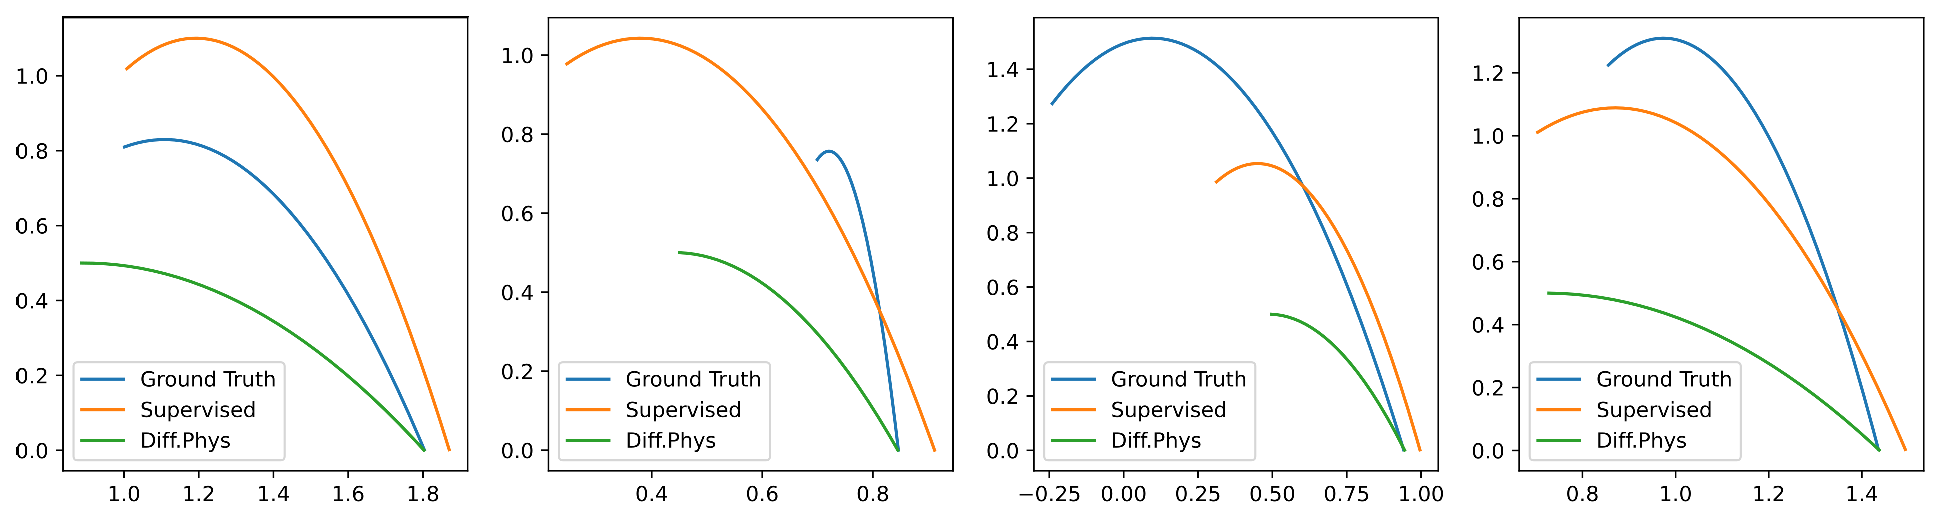
\includegraphics[width=\textwidth]{figures/throwing_results}
  \caption{Learning to throw. The goal is to give an initial velocity $v$, angle
    $\alpha$, and position $\vb{x}$ for a projectile, that hits a target at the
    ground floor when simulated.  The supervised network is outperformed by the
    \ac{DP} approach, as it always hits closer to the target by orders of
    magnitude than its supervised counterpart.  The only difference between the
    two agents being the way they derive their gradients from the same $L_2$
    error: while the \ac{DP} network gains an understanding of the underlying
    physical system via gradients of the simulation, the supervised network only
    sees examples of input-output pairs, where multimodality becomes an inherent
    problem.  (Figure recreated after [\cite{LearnToThrow}].)
  }
    \label{fig:learning-to-throw}
\end{figure}
